\chapterimage{media/headerLogo.png}
\chapter{Evaluierung und Diskussion der Ergebnisse}
\label{cha:ergebnisse}

\epigraph{No one learns as much about a subject as one who is forced to teach it.}{Peter F. Drucker}

\section{\autoref{cha:durchfuehrungfeature}: \nameref{cha:durchfuehrungfeature}}

\lipsum[3]

\newcommand{\specialcell}[2][c]{%
\begin{tabular}[#1]{@{}c@{}}#2\end{tabular}}

%%%%%%%%%%%%%
%%%% PH_KTC01
\begin{table}[!ht]
    \begin{subtable}{0.465\textwidth}
    \centering
        \resizebox{0.60\textwidth}{!}{%
        \begin{tabular}{cc|cc}
            \multicolumn{1}{c}{} &\multicolumn{1}{c}{} &\multicolumn{2}{c}{\scriptsize Vorhergesagt} \\ 
            \multicolumn{1}{c}{} & 
            \multicolumn{1}{c|}{} & 
            \multicolumn{1}{c}{Wahr} & 
            \multicolumn{1}{c}{Falsch} \\ \hline
            \multirow[c]{2}{*}{\rotatebox[origin=tr]{90}{\tiny Tatsächlich}}
            & Wahr      & 85     & 46     \\ [1.5ex]
            & Falsch    & 114    & 58    \\ \hline
        \end{tabular}
        }
        \caption{SAFE Confusion Matrix}
        \label{cmKTC01safe}
    \end{subtable}
    \hspace{0.2cm}
    \begin{subtable}{0.465\textwidth}
    \centering
        \resizebox{0.60\textwidth}{!}{%
        \begin{tabular}{cc|cc}
            \multicolumn{1}{c}{} &\multicolumn{1}{c}{} &\multicolumn{2}{c}{\scriptsize Vorhergesagt} \\ 
            \multicolumn{1}{c}{} & 
            \multicolumn{1}{c|}{} & 
            \multicolumn{1}{c}{Wahr} & 
            \multicolumn{1}{c}{Falsch} \\ \hline
            \multirow[c]{2}{*}{\rotatebox[origin=tr]{90}{\tiny Tatsächlich}}
            & Wahr      & 77    & 54     \\ [1.5ex]
            & Falsch    & 60    & 112    \\ \hline
        \end{tabular}
        }
        \caption{thesis Confusion Matrix}
        \label{cmKTC01thesis}
    \end{subtable}
    \vspace{0.1cm}
    \begin{subtable}{0.465\textwidth}
    \centering
        \resizebox{\textwidth}{!}{%
        \begin{tabular}{
        >{\columncolor[HTML]{FFFFFF}}r 
        >{\columncolor[HTML]{FFFFFF}}r 
        >{\columncolor[HTML]{FFFFFF}}r 
        >{\columncolor[HTML]{FFFFFF}}r 
        >{\columncolor[HTML]{FFFFFF}}r }
        \multicolumn{1}{l}{\cellcolor[HTML]{FFFFFF}} &
          \multicolumn{1}{l}{\cellcolor[HTML]{FFFFFF}precision} &
          \multicolumn{1}{l}{\cellcolor[HTML]{FFFFFF}recall} &
          \multicolumn{1}{l}{\cellcolor[HTML]{FFFFFF}f1-score} &
          \multicolumn{1}{l}{\cellcolor[HTML]{FFFFFF}support} \\ \cline{2-5} 
        \multicolumn{1}{r|}{\cellcolor[HTML]{FFFFFF}}             &      &      &      & \multicolumn{1}{r|}{\cellcolor[HTML]{FFFFFF}}    \\ \cline{1-1}
        \multicolumn{1}{|r}{\cellcolor[HTML]{FFFFFF}0}            & 0.55 & 0.34 & 0.42 & \multicolumn{1}{r|}{\cellcolor[HTML]{FFFFFF}171}  \\ \hline
        \multicolumn{1}{|r}{\cellcolor[HTML]{FFFFFF}1}            & 0.43 & 0.65 & 0.52 & \multicolumn{1}{r|}{\cellcolor[HTML]{FFFFFF}132}  \\ \hline
                                                                  &      &      &      &                                                  \\ \hline
        \multicolumn{1}{|r}{\cellcolor[HTML]{FFFFFF}accuray}      &      &      & 0.47 & \multicolumn{1}{r|}{\cellcolor[HTML]{FFFFFF}303} \\
        \multicolumn{1}{|r}{\cellcolor[HTML]{FFFFFF}macro avg}    & 0.33 & 0.33 & 0.31 & \multicolumn{1}{r|}{\cellcolor[HTML]{FFFFFF}303} \\
        \multicolumn{1}{|r}{\cellcolor[HTML]{FFFFFF}weighted avg} & 0.50 & 0.47 & 0.46 & \multicolumn{1}{r|}{\cellcolor[HTML]{FFFFFF}303} \\ \hline
        \end{tabular}%
        }
        \caption{SAFE POS-Muster}
        \label{csKTC01safe}
    \end{subtable}
    \hspace{0.2cm}
    \begin{subtable}{0.465\textwidth}
    \centering
        \resizebox{\textwidth}{!}{%
        \begin{tabular}{
        >{\columncolor[HTML]{FFFFFF}}r 
        >{\columncolor[HTML]{FFFFFF}}r 
        >{\columncolor[HTML]{FFFFFF}}r 
        >{\columncolor[HTML]{FFFFFF}}r 
        >{\columncolor[HTML]{FFFFFF}}r }
        \multicolumn{1}{l}{\cellcolor[HTML]{FFFFFF}} &
          \multicolumn{1}{l}{\cellcolor[HTML]{FFFFFF}precision} &
          \multicolumn{1}{l}{\cellcolor[HTML]{FFFFFF}recall} &
          \multicolumn{1}{l}{\cellcolor[HTML]{FFFFFF}f1-score} &
          \multicolumn{1}{l}{\cellcolor[HTML]{FFFFFF}support} \\ \cline{2-5} 
        \multicolumn{1}{r|}{\cellcolor[HTML]{FFFFFF}}             &      &      &      & \multicolumn{1}{r|}{\cellcolor[HTML]{FFFFFF}}    \\ \cline{1-1}
        \multicolumn{1}{|r}{\cellcolor[HTML]{FFFFFF}0}            & 0.67 & 0.65 & 0.66 & \multicolumn{1}{r|}{\cellcolor[HTML]{FFFFFF}171}  \\ \hline
        \multicolumn{1}{|r}{\cellcolor[HTML]{FFFFFF}1}            & 0.57 & 0.59 & 0.58 & \multicolumn{1}{r|}{\cellcolor[HTML]{FFFFFF}132}  \\ \hline
                                                                  &      &      &      &                                                  \\ \hline
        \multicolumn{1}{|r}{\cellcolor[HTML]{FFFFFF}accuray}      &      &      & 0.62 & \multicolumn{1}{r|}{\cellcolor[HTML]{FFFFFF}303} \\
        \multicolumn{1}{|r}{\cellcolor[HTML]{FFFFFF}macro avg}    & 0.41 & 0.41 & 0.41 & \multicolumn{1}{r|}{\cellcolor[HTML]{FFFFFF}303} \\
        \multicolumn{1}{|r}{\cellcolor[HTML]{FFFFFF}weighted avg} & 0.62 & 0.62 & 0.62 & \multicolumn{1}{r|}{\cellcolor[HTML]{FFFFFF}303} \\ \hline
        \end{tabular}%
        }
        \caption{thesis POS-Muster}
        \label{csKTC01thesis}
    \end{subtable}%
    \caption{Konfusionsmatrizen und Kennzahlen des PH\_KTC01}
    \label{tabs:resultsPHKTC01}
\end{table}

\lipsum[3]

\begin{figure}
     \centering
     \begin{subfigure}[b]{0.495\textwidth}
         \centering
         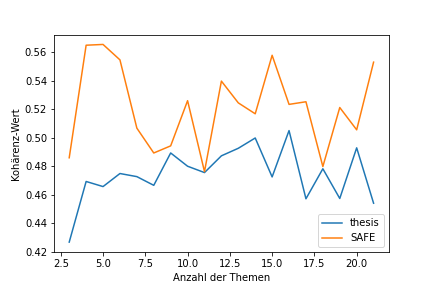
\includegraphics[width=\textwidth]{media/cs_PH_KTC01.png}
         \caption{PH\_KTC01}
         \label{fig:lda-ktc01}
     \end{subfigure}
     \hfill
     \begin{subfigure}[b]{0.495\textwidth}
         \centering
         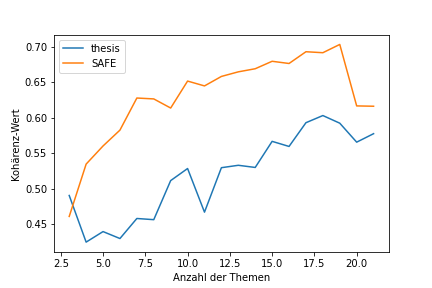
\includegraphics[width=\textwidth]{media/cs_PH_KTC02.png}
         \caption{PH\_KTC02}
         \label{fig:lda-ktc02}
     \end{subfigure}
    \caption{Ergebnisse der Themenmodellierung: PH\_KTC01-02}
    \label{figs:tmtopiccoherence}
\end{figure}

\lipsum[1]

\section{Diskussion}
\label{sec:diskussion}

\lipsum[3]
